\documentclass{beamer}
\usepackage[utf8]{inputenc}
\usetheme{default}
\usecolortheme{dove}
\usepackage{textpos}
\usepackage{grid-system}

% po4a: environment frame
% po4a: environment Row
% po4a: environment Cell


\title{Freifunk Darmstadt}
\author{
\includegraphics[width=4cm]{images/logo}}
%\institute[Inst.]{Freifunk Darmstadt}
\date{29. Januar 2014}

\begin{document}

\begin{frame}
\maketitle
\end{frame}

\addtobeamertemplate{frametitle}{}{%
\begin{textblock*}{100mm}(0.93\textwidth,-0.5cm)

\includegraphics[height=1cm]{images/logo}
\end{textblock*}}

\begin{frame}{Outline}
\tableofcontents
\end{frame}

\section{Einleitung}
\begin{frame}{Einleitung}
\end{frame}

\section{Projektbeschreibung}
\begin{frame}{Projektbeschreibung}
\end{frame}

\section{Aktueller Stand}
\begin{frame}{Aktueller Stand}
Wie viele und welche Standorte sind derzeit abgedeckt?
\end{frame}

\section{Ausbauplan}
\begin{frame}{}
Gibt es einen Ausbauplan?
\end{frame}

\section{Accesspoints}
\begin{frame}{Accesspoints}
Gibt es outdoor-fähige Accesspoints?
\end{frame}

\section{Beispiel Luisenplatz}
\begin{frame}{Beispiel: Luisenplatz}
Wie sieht die Leistungsfähigkeit der technischen Lösung am Beispiel Luisenplatz aus?
\end{frame}

\section{Anforderungen an die Stadt}
\begin{frame}{Anforderungen an die Stadt}
Was sind die Anforderungen an die Stadt für eine gemeinsame Kooperation?
Welche Kosten entstehen für die Stadt Darmstadt?
\end{frame}

\section{Betrieb}
\begin{frame}{Betrieb}
Wie wird der Betrieb sichergestellt?
Ist ein durchgehender Betrieb sichergestellt?
Welche Reaktionszeiten/Wiederherstellungszeiten werden garantiert?
\end{frame}










\begin{frame}{Weitere Fragen?}
\vfill
\centering
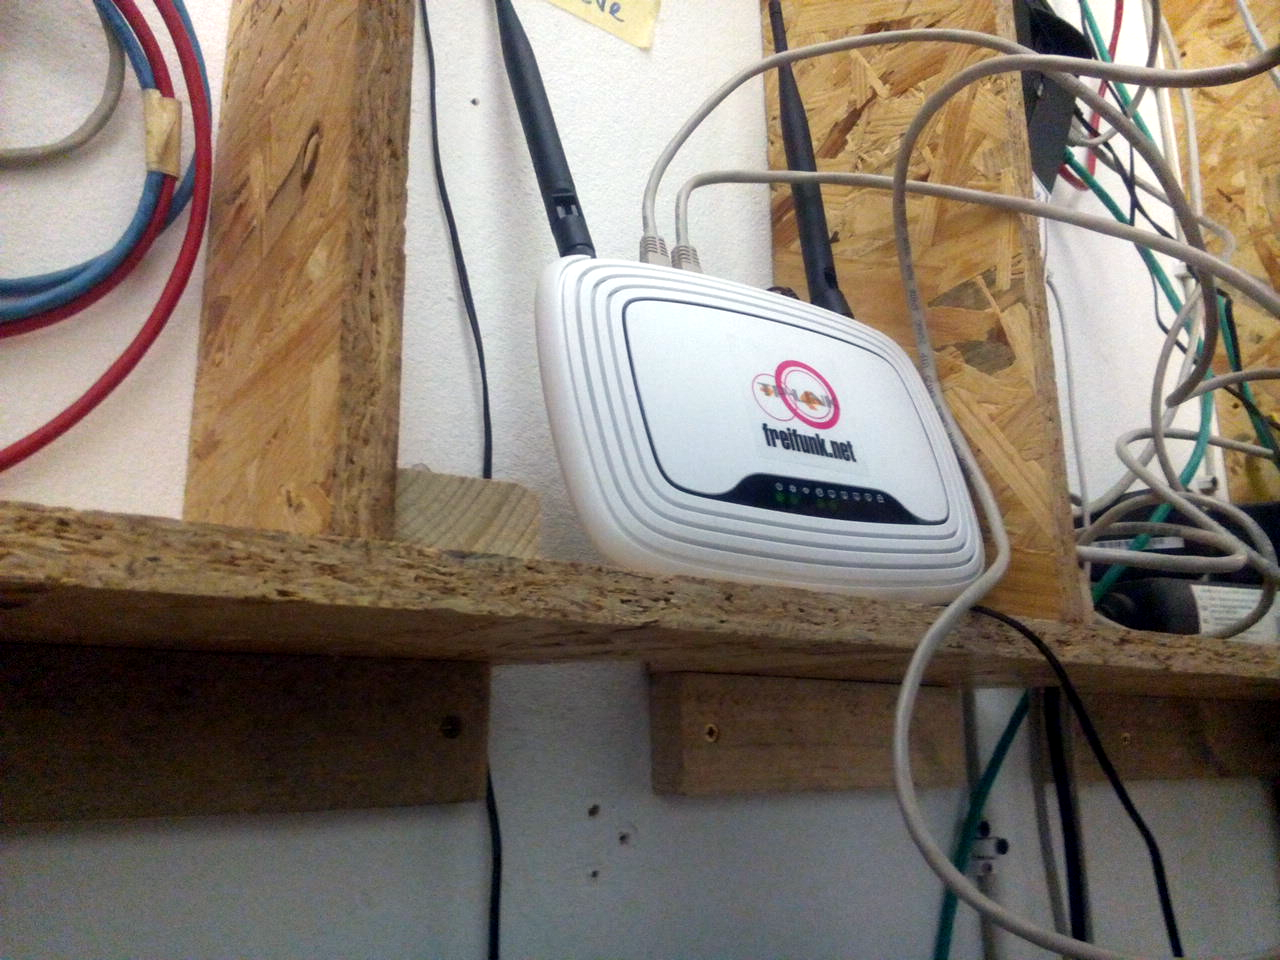
\includegraphics[width=0.7\textwidth]{images/irl_router}
\vfill
\end{frame}


\end{document}
